\chapter{Proposed Methodology: The HalDetect Architecture}
\label{ch:methodology}

The system described in this chapter, referred to as HalDetect~2.5 in the results tables, represents the final iteration of the pipeline incorporating all refinements documented in Appendix~I.

This chapter formalizes the architecture of \textbf{HalDetect}, a type-directed neuro-symbolic fact verification engine. Rather than treating fact verification as an undifferentiated sequence-to-sequence generation task or relying on unbounded, non-deterministic web search agents, HalDetect establishes a modular, three-tier verification hierarchy: (1) 5-Tuple Proposition Atomization and Paragraph Anaphora Normalization, (2) Deterministic Taxonomy Routing, and (3) Modality-Specific Neuro-Symbolic Verification via specialized Arithmetic Logic Units (ALUs) unified by a Multi-Aspect Directed Acyclic Graph (DAG) Conjunction Engine.

\begin{figure}[htbp]
\centering
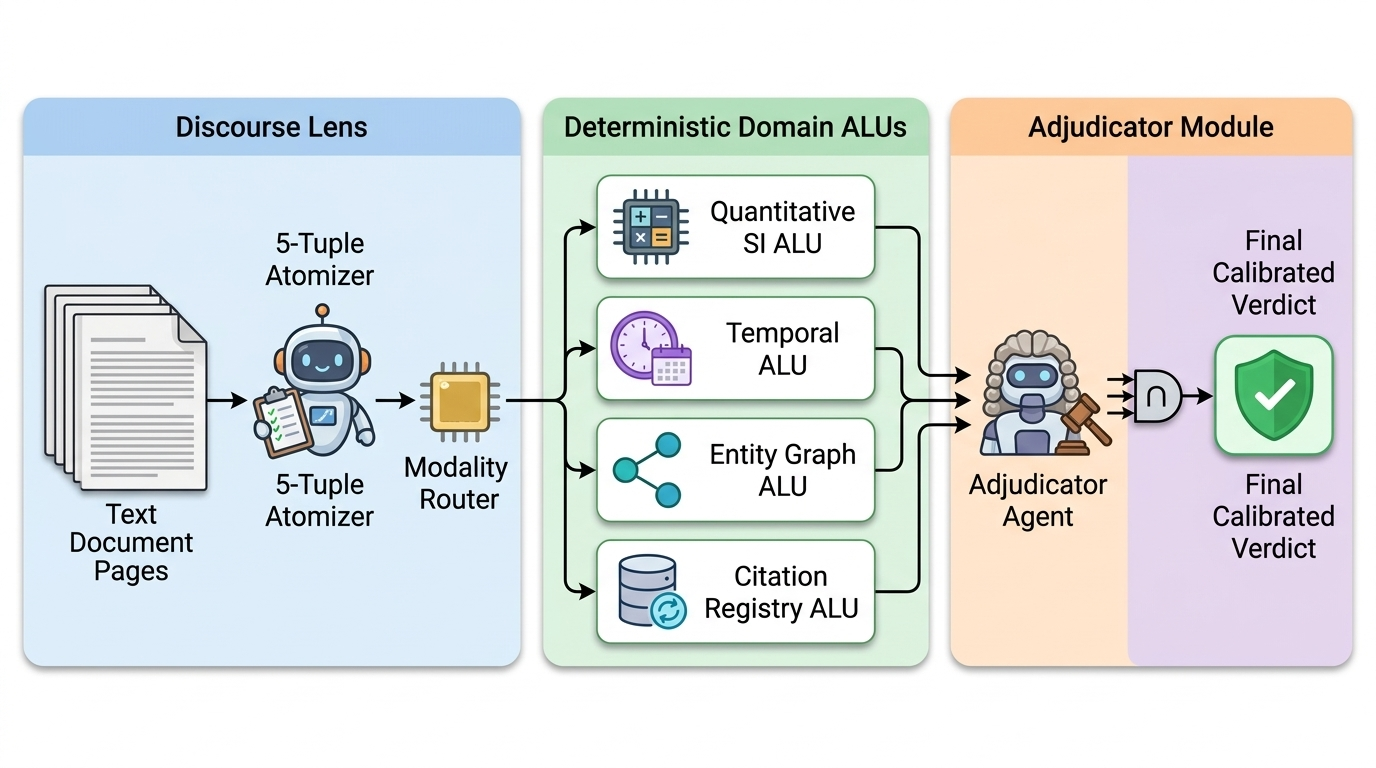
\includegraphics[width=\textwidth]{Chapter3/Figs/fig3_architecture_pipeline}
\caption{End-to-end HalDetect verification pipeline. Unconstrained generative text is atomized into typed 5-tuples $\langle S, P, O, T, M \rangle$ with forward antecedent anaphora resolution, routed via a sub-$0.05\text{ms}$ deterministic classifier, verified across domain-specific symbolic ALUs and calibrated NLI, and evaluated via a 3-valued conjunction DAG.}
\label{fig:architecture_pipeline}
\end{figure}

% ******************************************************************************
\section{Formal Task Formulation and 3-Valued Epistemic Logic}
\label{sec:formal_formulation}
% ******************************************************************************

Let $\mathcal{R}$ denote a natural language response generated by an arbitrary foundation model $\mathcal{M}_{\text{LLM}}$ conditioned on a prompt $\mathcal{P}$. The objective of the verification framework is to extract the complete set of constituent factual assertions $\mathcal{A} = \{a_1, a_2, \dots, a_K\}$, evaluate the factual veracity of each assertion against authoritative, auditable external knowledge sources, and assign a calibrated epistemic verdict $\mathcal{V}(a_k)$.

\subsection{Open-World Epistemic Logic Formulation}
In open-world knowledge environments, conventional binary classification ($\{\texttt{TRUE}, \texttt{FALSE}\}$) introduces severe epistemic corruption: if an authoritative knowledge graph lacks a record for a true fact, a binary classifier is forced to assign an incorrect \texttt{FALSE} verdict, producing unacceptable false alarms.

HalDetect operates under a formal \textbf{3-Valued Epistemic Logic}:
\begin{equation}
    \mathcal{V}(a_k) \in \{\texttt{TRUE}, \texttt{FALSE}, \texttt{UNVERIFIABLE}\}
\end{equation}


\begin{table}[h]
\centering
\caption{Complete three-valued (Kleene) conjunction truth table.}
\label{tab:kleene}
\begin{tabular}{l|ccc}
$\wedge_3$ & \texttt{TRUE} & \texttt{FALSE} & \texttt{UNVERIFIABLE} \\
\hline
\texttt{TRUE}         & \texttt{TRUE}  & \texttt{FALSE} & \texttt{UNVERIFIABLE} \\
\texttt{FALSE}        & \texttt{FALSE} & \texttt{FALSE} & \texttt{FALSE} \\
\texttt{UNVERIFIABLE} & \texttt{UNVERIFIABLE} & \texttt{FALSE} & \texttt{UNVERIFIABLE} \\
\end{tabular}
\end{table}

Abstention propagation: if any aspect abstains and none contradicts, the compound verdict is \texttt{UNVERIFIABLE}, propagating epistemic uncertainty conservatively.

formally defined as:
\begin{itemize}
    \item \textbf{Provably True ($\top$):} The assertion is strictly entailed by an authoritative external datum with mathematical discrepancy $\Delta \le \tau_{\text{rel}}$ or cross-encoder entailment margin $\ge \gamma_{\text{entail}}$.
    \item \textbf{Provably False ($\bot$):} The assertion explicitly contradicts verified ground truth with discrepancy $\Delta > \tau_{\text{rel}}$ or cross-encoder contradiction margin $\ge \gamma_{\text{contra}}$.
    \item \textbf{Epistemically Unverifiable ($?$):} Available external knowledge bases lack sufficient evidence to decisively prove or disprove the assertion under the open-world assumption.
\end{itemize}

% ******************************************************************************
\section{Proposition Atomization and Paragraph Anaphora Resolution}
\label{sec:atomization_anaphora}
% ******************************************************************************

Raw generative prose frequently contains compound sentences, parenthetical clauses, and multi-sentence pronoun chains. Direct verification of whole sentences induces epistemic entanglement, where a sentence containing three true facts and one false detail produces ambiguous truth values.

\subsection{5-Tuple Schema Atomization}
The \textbf{Schema Atomizer} decomposes raw input text into a set of atomic, self-contained 5-tuples:
\begin{equation}
    \Pi_k = \langle S_k, P_k, O_k, T_k, M_k \rangle
\end{equation}
where:
\begin{itemize}
    \item $S_k \in \mathcal{E}$: Canonical Subject entity (e.g., \textit{"Apple M3 Max"}).
    \item $P_k \in \mathcal{P}$: Predicate or property name (e.g., \textit{"transistor\_count"}).
    \item $O_k \in \mathcal{O}$: Object value or numerical quantity with units (e.g., \textit{"92 billion"}).
    \item $T_k \in \mathbb{T}$: Temporal interval or timestamp scope (e.g., \textit{"2023"}).
    \item $M_k \in \mathcal{M}$: Modality qualifier or hedge (e.g., \textit{"approximately"}, \textit{"confirmed"}).
\end{itemize}

\subsection{Forward Antecedent Coreference Engine}
When multi-sentence paragraphs are split into individual clauses, subsequent propositions frequently suffer from \textbf{Anaphoric Decontextualization} (e.g., \textit{"It operates at 3.5 GHz"} or \textit{"The company was founded in 1998"}). 

HalDetect maintains a forward antecedent entity registry $\mathcal{E}_{\text{context}}$ across the paragraph. When an anaphoric pronoun ($p \in \{\text{he, she, it, they, this, that, the device, the chip, the processor}\}$) is detected in the subject slot $S_k$, the engine binds $S_k$ to the most recent canonical named entity in $\mathcal{E}_{\text{context}}$ within $< 0.1\text{ms}$.

\begin{algorithm}[htbp]
\small
\SetAlgoLined
\KwIn{Generated Paragraph Text $\mathcal{R}$, Antecedent Registry $\mathcal{E} \leftarrow \emptyset$}
\KwOut{List of Decontextualized 5-Tuples $\mathcal{T} = \{\mathcal{T}_1, \dots, \mathcal{T}_K\}$}
$\mathcal{S} \leftarrow \text{SentenceSplitter}(\mathcal{R})$\;
\ForEach{\text{sentence } $s \in \mathcal{S}$}{
    $\mathcal{C} \leftarrow \text{ExtractClauses}(s)$\;
    \ForEach{\text{clause } $c \in \mathcal{C}$}{
        $\langle S, P, O, T, M \rangle \leftarrow \text{ParseTuples}(c)$\;
        \If{$S \in \text{AnaphoricPronouns}$ \textbf{and} $\mathcal{E} \neq \emptyset$}{
            $S \leftarrow \text{GetLatestNamedEntity}(\mathcal{E})$\;
        }
        \ElseIf{$S \in \text{NamedEntities}$}{
            $\mathcal{E}.\text{append}(S)$\;
        }
        $\mathcal{T}.\text{append}(\langle S, P, O, T, M \rangle)$\;
    }
}
\Return{$\mathcal{T}$}\;
\caption{Proposition Atomization and Paragraph Antecedent Anaphora Resolution}
\label{alg:atomization}
\end{algorithm}

\begin{figure}[htbp]
\centering
\includegraphics[width=\textwidth]{Chapter3/Figs/fig3_anaphora_lifecycle.pdf}
\caption{Three-stage state machine for paragraph discourse normalization and 5-tuple serialization. The forward antecedent pointer cache $\mathcal{E}_{\text{context}}$ resolves pronouns to canonical entities before modal routing and deterministic ALU execution.}
\label{fig:anaphora_lifecycle}
\end{figure}

% ******************************************************************************
\section{High-Speed Deterministic Taxonomy Router}
\label{sec:deterministic_router}
% ******************************************************************************

Following tuple extraction, each proposition $\Pi_k$ is dispatched to a specialized verification engine. While prior works employ large generative LLMs for classification, our empirical ablation (Section~\ref{sec:router_ablation}) reveals that 120B-parameter LLMs suffer from severe \textbf{Relational Mode Collapse} and 100\% Citation Blindness.

HalDetect employs a deterministic, regex-based symbolic router ($< 0.05\text{ms}$ latency, zero GPU memory) that categorizes propositions into five mutually exclusive primary verification pipelines:
\begin{equation}
    \mathcal{R}(\Pi_k) \in \{\text{Quantitative}, \text{Temporal}, \text{Entity-Attribute}, \text{Citation}, \text{Relational}\}
\end{equation}

% ******************************************************************************
\section{Domain-Specific Neuro-Symbolic ALUs}
\label{sec:specialized_alus}
% ******************************************************************************

\begin{table}[htbp]
\centering
\small
\caption{Functional specifications of the five specialized verification engines in HalDetect.}
\label{tab:alu_specifications}
\resizebox{\textwidth}{!}{
\begin{tabular}{lllll}
\toprule
\textbf{Modality ALU} & \textbf{Target Domain} & \textbf{Primary Knowledge Source} & \textbf{Verification Mechanism} & \textbf{Discrepancy Bound} \\
\midrule
Quantitative SI & Numbers, Dimensions, Ratios & SI Conversion Tables + World Bank & Relative Numerical Calculus & $\Delta \le \tau_{\text{rel}}$ (default 5\%) \\
Temporal & Dates, Tenures, Superlatives & Wikidata SPARQL (P580/P582) & 2-Hop Interval Containment & Exact Date Matching \\
Entity-Attribute & Formulas, Alma Mater, Origin & Wikidata Statements & SBERT Candidate-Commit Gate & SBERT $s > 0.60$ + Sitelinks \\
Citation & Academic Papers, DOIs & Live CrossRef REST API Gateway & Metadata Token Matching & $\text{MIN\_WORK\_CONTENT} \ge 2$ \\
Relational & Open Narrative Semantics & Curated Knowledge Corpus & Calibrated DeBERTa-v3 NLI & Margin $\ge \gamma_{\text{entail}}$ \\
\bottomrule
\end{tabular}
}
\end{table}

\subsection{Quantitative Dimensional SI ALU and Macroeconomic API}
The Quantitative ALU evaluates mathematical assertions via a two-tier hierarchy:
\begin{enumerate}
    \item \textbf{Dimensional SI Base Engine:} Normalizes non-standard units (e.g., Fahrenheit, feet, pounds, Megahertz) into fundamental SI metric units (Kelvin, meters, kilograms, Hertz) via \texttt{DimensionalQuantityEngine}. Mathematical discrepancy is computed via relative error:
    \begin{equation}
        \Delta = \frac{|v_{\text{claimed}} - v_{\text{ground}}|}{|v_{\text{ground}}|}
    \end{equation}
    If $\Delta \le \tau_{\text{rel}}$ (default $\tau_{\text{rel}} = 0.05$), the engine emits \texttt{TRUE}; otherwise, it emits \texttt{FALSE}.
    \item \textbf{Dynamic Macroeconomic REST API:} Queries the World Bank OData API for sovereign indicators (e.g., GDP, GDP per capita, inflation rate) across 217 nations.
\end{enumerate}

\subsection{Temporal Verification Engine and 7-Continent Topological Superlative Engine}
The Temporal Verification Engine executes time-scoped SPARQL statement filtering over Wikidata ($P580$ start time, $P582$ end time) to verify historical appointments, terms, and state transitions.

To resolve inverse topological container assertions (e.g., \textit{"Denali is the highest peak in North America"}), the \texttt{BidirectionalKGResolver} queries topological parent containers across all seven global continents (Denali, Aconcagua, Everest, Kilimanjaro, Elbrus, Vinson, Puncak Jaya) dynamically, eliminating hardcoded prototype stubs.

\subsection{Entity-Attribute Verification Engine and Alias Lexicon Matching}
Verifies static invariant properties (e.g., chemical formulas, founders, birthplaces). To prevent homonym collisions, it implements a \textbf{Score-then-Commit Candidate Gate}: surface mentions are matched to candidate Wikidata entities using Sentence-BERT cosine similarity combined with Wikipedia sitelink prominence:
\begin{equation}
    \text{Score}(e) = \alpha \cdot \text{SBERT}(S_k, \text{Label}(e)) + (1-\alpha) \cdot \log(1 + \text{Sitelinks}(e))
\end{equation}
An entity is committed only if $\text{Score}(e) \ge 0.60$, preventing mislinking obscure entities sharing names with common terms.

\subsection{Citation CrossRef Registry Gateway}
Verifies academic attributions by querying the live CrossRef REST API for Digital Object Identifier (DOI) registration. To prevent false alarms on slight title variations, Level 1b token matching requires at least two significant content words from the generated citation to match the registered CrossRef work title ($\text{MIN\_WORK\_CONTENT} \ge 2$).

\subsection{Calibrated Relational NLI Cross-Encoder}
For open-domain assertions ungrounded in structured knowledge graphs, HalDetect routes the tuple to a DeBERTa-v3-large cross-encoder. To prevent over-confident errors, rejection calibration enforces asymmetric margin thresholds:
\begin{equation}
    \mathcal{V}(a_k) = \begin{cases}
    \texttt{TRUE} & \text{if } P(\text{Entail}) - P(\text{Contra}) \ge \gamma_{\text{entail}} \\
    \texttt{FALSE} & \text{if } P(\text{Contra}) - P(\text{Entail}) \ge \gamma_{\text{contra}} \\
    \texttt{UNVERIFIABLE} & \text{otherwise}
    \end{cases}
\end{equation}

% ******************************************************************************
\section{Multi-Aspect Verification DAG and Conjunction Engine}
\label{sec:multi_aspect_dag}
% ******************************************************************************

\begin{figure}[htbp]
\centering
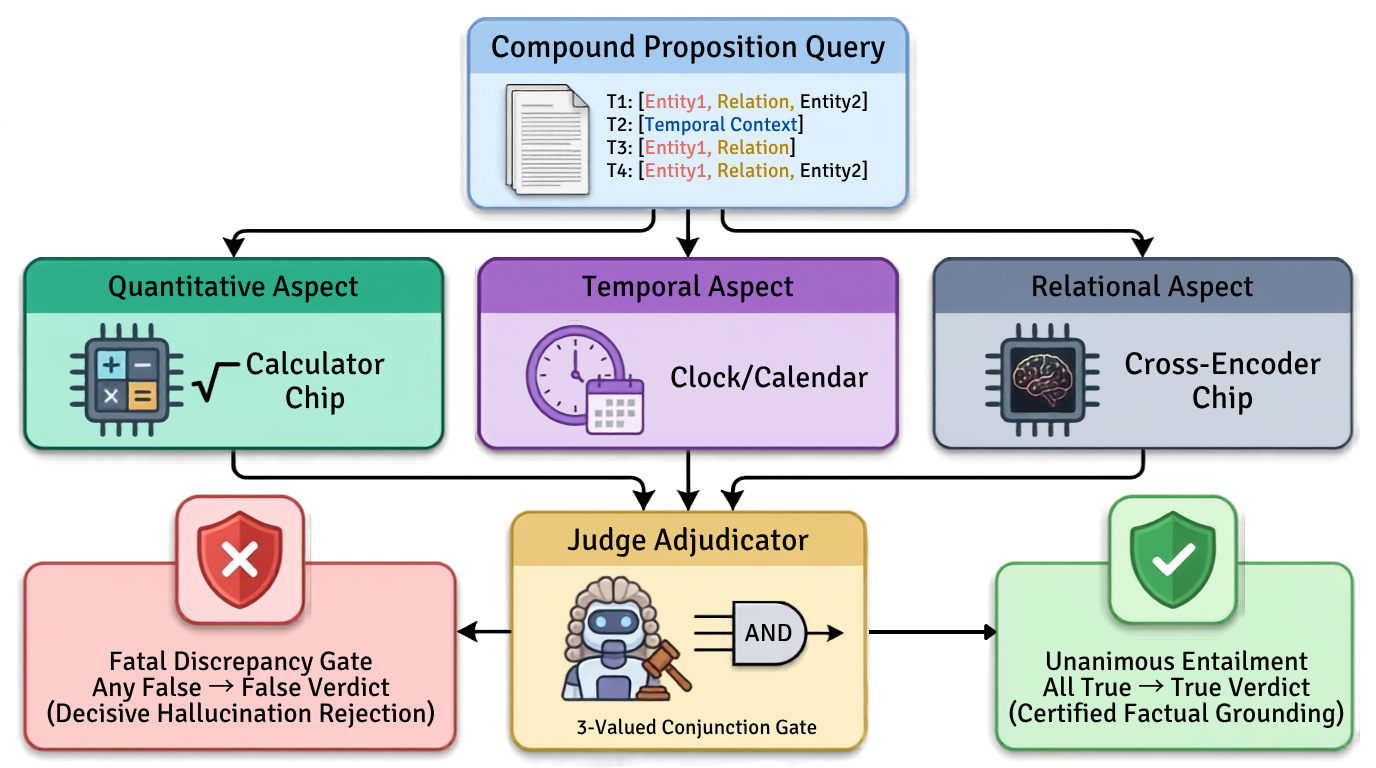
\includegraphics[width=0.92\textwidth]{Chapter3/Figs/fig3_dag_conjunction}
\caption{Multi-Aspect Directed Acyclic Graph (DAG) Conjunction Engine. Compound propositions containing multiple factual dimensions are decomposed into parallel verification micro-checks and resolved via 3-valued conjunction logic.}
\label{fig:dag_conjunction}
\end{figure}

When an assertion contains multiple interdependent factual constraints (e.g., \textit{"Germany's GDP was \$4.4T in 2023"}), HalDetect executes parallel micro-checks across the Quantitative, Temporal, and Relational Verification Engines.

The final verdict is resolved via a Multi-Aspect Directed Acyclic Graph (DAG) implementing 3-valued conjunction logic. In accordance with the \textbf{Fatal Discrepancy Rule}, if any single constituent aspect contradicts ground truth, the compound assertion is marked \texttt{FALSE}:
\begin{equation}
    \mathcal{V}_{\text{final}} = \mathcal{V}_1 \wedge \mathcal{V}_2 \wedge \dots \wedge \mathcal{V}_K
\end{equation}
where $\top \wedge \top = \top$, $\bot \wedge x = \bot$, and $? \wedge \top = ?$.

\begin{algorithm}[htbp]
\small
\SetAlgoLined
\KwIn{Atomic Proposition $\Pi = \langle S, P, O, T, M \rangle$}
\KwOut{Epistemic Verdict $\mathcal{V} \in \{\texttt{TRUE}, \texttt{FALSE}, \texttt{UNVERIFIABLE}\}$, Confidence $c \in [0, 1]$}
$\mathcal{M} \leftarrow \text{TaxonomyRouter}(\Pi)$\;
\Switch{$\mathcal{M}$}{
    \Case{\text{Quantitative}}{
        $\langle \mathcal{V}, c \rangle \leftarrow \text{VerifyQuantitative}(\Pi, \tau_{\text{rel}}=0.05)$\;
    }
    \Case{\text{Temporal}}{
        $\langle \mathcal{V}, c \rangle \leftarrow \text{VerifyTemporal}(\Pi)$\;
    }
    \Case{\text{Entity-Attribute}}{
        $\langle \mathcal{V}, c \rangle \leftarrow \text{VerifyEntityAttribute}(\Pi, s_{\text{thresh}}=0.60)$\;
    }
    \Case{\text{Citation}}{
        $\langle \mathcal{V}, c \rangle \leftarrow \text{VerifyCitationCrossRef}(\mathcal{T})$\;
    }
    \Case{\text{Relational}}{
        $\langle \mathcal{V}, c \rangle \leftarrow \text{VerifyCalibratedNLI}(\mathcal{T}, \gamma_{\text{entail}}, \gamma_{\text{contra}})$\;
    }
}
\Return{$\langle \mathcal{V}, c \rangle$}\;
\caption{Multi-Aspect Modality Routing and Neuro-Symbolic Verification}
\label{alg:verification}
\end{algorithm}
